% Options for packages loaded elsewhere
\PassOptionsToPackage{unicode}{hyperref}
\PassOptionsToPackage{hyphens}{url}
\PassOptionsToPackage{dvipsnames,svgnames,x11names}{xcolor}
%
\documentclass[
  letterpaper,
  DIV=11,
  numbers=noendperiod]{scrreprt}

\usepackage{amsmath,amssymb}
\usepackage{iftex}
\ifPDFTeX
  \usepackage[T1]{fontenc}
  \usepackage[utf8]{inputenc}
  \usepackage{textcomp} % provide euro and other symbols
\else % if luatex or xetex
  \usepackage{unicode-math}
  \defaultfontfeatures{Scale=MatchLowercase}
  \defaultfontfeatures[\rmfamily]{Ligatures=TeX,Scale=1}
\fi
\usepackage{lmodern}
\ifPDFTeX\else  
    % xetex/luatex font selection
\fi
% Use upquote if available, for straight quotes in verbatim environments
\IfFileExists{upquote.sty}{\usepackage{upquote}}{}
\IfFileExists{microtype.sty}{% use microtype if available
  \usepackage[]{microtype}
  \UseMicrotypeSet[protrusion]{basicmath} % disable protrusion for tt fonts
}{}
\makeatletter
\@ifundefined{KOMAClassName}{% if non-KOMA class
  \IfFileExists{parskip.sty}{%
    \usepackage{parskip}
  }{% else
    \setlength{\parindent}{0pt}
    \setlength{\parskip}{6pt plus 2pt minus 1pt}}
}{% if KOMA class
  \KOMAoptions{parskip=half}}
\makeatother
\usepackage{xcolor}
\setlength{\emergencystretch}{3em} % prevent overfull lines
\setcounter{secnumdepth}{5}
% Make \paragraph and \subparagraph free-standing
\ifx\paragraph\undefined\else
  \let\oldparagraph\paragraph
  \renewcommand{\paragraph}[1]{\oldparagraph{#1}\mbox{}}
\fi
\ifx\subparagraph\undefined\else
  \let\oldsubparagraph\subparagraph
  \renewcommand{\subparagraph}[1]{\oldsubparagraph{#1}\mbox{}}
\fi

\usepackage{color}
\usepackage{fancyvrb}
\newcommand{\VerbBar}{|}
\newcommand{\VERB}{\Verb[commandchars=\\\{\}]}
\DefineVerbatimEnvironment{Highlighting}{Verbatim}{commandchars=\\\{\}}
% Add ',fontsize=\small' for more characters per line
\usepackage{framed}
\definecolor{shadecolor}{RGB}{241,243,245}
\newenvironment{Shaded}{\begin{snugshade}}{\end{snugshade}}
\newcommand{\AlertTok}[1]{\textcolor[rgb]{0.68,0.00,0.00}{#1}}
\newcommand{\AnnotationTok}[1]{\textcolor[rgb]{0.37,0.37,0.37}{#1}}
\newcommand{\AttributeTok}[1]{\textcolor[rgb]{0.40,0.45,0.13}{#1}}
\newcommand{\BaseNTok}[1]{\textcolor[rgb]{0.68,0.00,0.00}{#1}}
\newcommand{\BuiltInTok}[1]{\textcolor[rgb]{0.00,0.23,0.31}{#1}}
\newcommand{\CharTok}[1]{\textcolor[rgb]{0.13,0.47,0.30}{#1}}
\newcommand{\CommentTok}[1]{\textcolor[rgb]{0.37,0.37,0.37}{#1}}
\newcommand{\CommentVarTok}[1]{\textcolor[rgb]{0.37,0.37,0.37}{\textit{#1}}}
\newcommand{\ConstantTok}[1]{\textcolor[rgb]{0.56,0.35,0.01}{#1}}
\newcommand{\ControlFlowTok}[1]{\textcolor[rgb]{0.00,0.23,0.31}{#1}}
\newcommand{\DataTypeTok}[1]{\textcolor[rgb]{0.68,0.00,0.00}{#1}}
\newcommand{\DecValTok}[1]{\textcolor[rgb]{0.68,0.00,0.00}{#1}}
\newcommand{\DocumentationTok}[1]{\textcolor[rgb]{0.37,0.37,0.37}{\textit{#1}}}
\newcommand{\ErrorTok}[1]{\textcolor[rgb]{0.68,0.00,0.00}{#1}}
\newcommand{\ExtensionTok}[1]{\textcolor[rgb]{0.00,0.23,0.31}{#1}}
\newcommand{\FloatTok}[1]{\textcolor[rgb]{0.68,0.00,0.00}{#1}}
\newcommand{\FunctionTok}[1]{\textcolor[rgb]{0.28,0.35,0.67}{#1}}
\newcommand{\ImportTok}[1]{\textcolor[rgb]{0.00,0.46,0.62}{#1}}
\newcommand{\InformationTok}[1]{\textcolor[rgb]{0.37,0.37,0.37}{#1}}
\newcommand{\KeywordTok}[1]{\textcolor[rgb]{0.00,0.23,0.31}{#1}}
\newcommand{\NormalTok}[1]{\textcolor[rgb]{0.00,0.23,0.31}{#1}}
\newcommand{\OperatorTok}[1]{\textcolor[rgb]{0.37,0.37,0.37}{#1}}
\newcommand{\OtherTok}[1]{\textcolor[rgb]{0.00,0.23,0.31}{#1}}
\newcommand{\PreprocessorTok}[1]{\textcolor[rgb]{0.68,0.00,0.00}{#1}}
\newcommand{\RegionMarkerTok}[1]{\textcolor[rgb]{0.00,0.23,0.31}{#1}}
\newcommand{\SpecialCharTok}[1]{\textcolor[rgb]{0.37,0.37,0.37}{#1}}
\newcommand{\SpecialStringTok}[1]{\textcolor[rgb]{0.13,0.47,0.30}{#1}}
\newcommand{\StringTok}[1]{\textcolor[rgb]{0.13,0.47,0.30}{#1}}
\newcommand{\VariableTok}[1]{\textcolor[rgb]{0.07,0.07,0.07}{#1}}
\newcommand{\VerbatimStringTok}[1]{\textcolor[rgb]{0.13,0.47,0.30}{#1}}
\newcommand{\WarningTok}[1]{\textcolor[rgb]{0.37,0.37,0.37}{\textit{#1}}}

\providecommand{\tightlist}{%
  \setlength{\itemsep}{0pt}\setlength{\parskip}{0pt}}\usepackage{longtable,booktabs,array}
\usepackage{calc} % for calculating minipage widths
% Correct order of tables after \paragraph or \subparagraph
\usepackage{etoolbox}
\makeatletter
\patchcmd\longtable{\par}{\if@noskipsec\mbox{}\fi\par}{}{}
\makeatother
% Allow footnotes in longtable head/foot
\IfFileExists{footnotehyper.sty}{\usepackage{footnotehyper}}{\usepackage{footnote}}
\makesavenoteenv{longtable}
\usepackage{graphicx}
\makeatletter
\def\maxwidth{\ifdim\Gin@nat@width>\linewidth\linewidth\else\Gin@nat@width\fi}
\def\maxheight{\ifdim\Gin@nat@height>\textheight\textheight\else\Gin@nat@height\fi}
\makeatother
% Scale images if necessary, so that they will not overflow the page
% margins by default, and it is still possible to overwrite the defaults
% using explicit options in \includegraphics[width, height, ...]{}
\setkeys{Gin}{width=\maxwidth,height=\maxheight,keepaspectratio}
% Set default figure placement to htbp
\makeatletter
\def\fps@figure{htbp}
\makeatother
% definitions for citeproc citations
\NewDocumentCommand\citeproctext{}{}
\NewDocumentCommand\citeproc{mm}{%
  \begingroup\def\citeproctext{#2}\cite{#1}\endgroup}
\makeatletter
 % allow citations to break across lines
 \let\@cite@ofmt\@firstofone
 % avoid brackets around text for \cite:
 \def\@biblabel#1{}
 \def\@cite#1#2{{#1\if@tempswa , #2\fi}}
\makeatother
\newlength{\cslhangindent}
\setlength{\cslhangindent}{1.5em}
\newlength{\csllabelwidth}
\setlength{\csllabelwidth}{3em}
\newenvironment{CSLReferences}[2] % #1 hanging-indent, #2 entry-spacing
 {\begin{list}{}{%
  \setlength{\itemindent}{0pt}
  \setlength{\leftmargin}{0pt}
  \setlength{\parsep}{0pt}
  % turn on hanging indent if param 1 is 1
  \ifodd #1
   \setlength{\leftmargin}{\cslhangindent}
   \setlength{\itemindent}{-1\cslhangindent}
  \fi
  % set entry spacing
  \setlength{\itemsep}{#2\baselineskip}}}
 {\end{list}}
\usepackage{calc}
\newcommand{\CSLBlock}[1]{\hfill\break\parbox[t]{\linewidth}{\strut\ignorespaces#1\strut}}
\newcommand{\CSLLeftMargin}[1]{\parbox[t]{\csllabelwidth}{\strut#1\strut}}
\newcommand{\CSLRightInline}[1]{\parbox[t]{\linewidth - \csllabelwidth}{\strut#1\strut}}
\newcommand{\CSLIndent}[1]{\hspace{\cslhangindent}#1}

\KOMAoption{captions}{tableheading}
\makeatletter
\@ifpackageloaded{tcolorbox}{}{\usepackage[skins,breakable]{tcolorbox}}
\@ifpackageloaded{fontawesome5}{}{\usepackage{fontawesome5}}
\definecolor{quarto-callout-color}{HTML}{909090}
\definecolor{quarto-callout-note-color}{HTML}{0758E5}
\definecolor{quarto-callout-important-color}{HTML}{CC1914}
\definecolor{quarto-callout-warning-color}{HTML}{EB9113}
\definecolor{quarto-callout-tip-color}{HTML}{00A047}
\definecolor{quarto-callout-caution-color}{HTML}{FC5300}
\definecolor{quarto-callout-color-frame}{HTML}{acacac}
\definecolor{quarto-callout-note-color-frame}{HTML}{4582ec}
\definecolor{quarto-callout-important-color-frame}{HTML}{d9534f}
\definecolor{quarto-callout-warning-color-frame}{HTML}{f0ad4e}
\definecolor{quarto-callout-tip-color-frame}{HTML}{02b875}
\definecolor{quarto-callout-caution-color-frame}{HTML}{fd7e14}
\makeatother
\makeatletter
\@ifpackageloaded{bookmark}{}{\usepackage{bookmark}}
\makeatother
\makeatletter
\@ifpackageloaded{caption}{}{\usepackage{caption}}
\AtBeginDocument{%
\ifdefined\contentsname
  \renewcommand*\contentsname{Table of contents}
\else
  \newcommand\contentsname{Table of contents}
\fi
\ifdefined\listfigurename
  \renewcommand*\listfigurename{List of Figures}
\else
  \newcommand\listfigurename{List of Figures}
\fi
\ifdefined\listtablename
  \renewcommand*\listtablename{List of Tables}
\else
  \newcommand\listtablename{List of Tables}
\fi
\ifdefined\figurename
  \renewcommand*\figurename{Figure}
\else
  \newcommand\figurename{Figure}
\fi
\ifdefined\tablename
  \renewcommand*\tablename{Table}
\else
  \newcommand\tablename{Table}
\fi
}
\@ifpackageloaded{float}{}{\usepackage{float}}
\floatstyle{ruled}
\@ifundefined{c@chapter}{\newfloat{codelisting}{h}{lop}}{\newfloat{codelisting}{h}{lop}[chapter]}
\floatname{codelisting}{Listing}
\newcommand*\listoflistings{\listof{codelisting}{List of Listings}}
\makeatother
\makeatletter
\makeatother
\makeatletter
\@ifpackageloaded{caption}{}{\usepackage{caption}}
\@ifpackageloaded{subcaption}{}{\usepackage{subcaption}}
\makeatother
\ifLuaTeX
  \usepackage{selnolig}  % disable illegal ligatures
\fi
\usepackage{bookmark}

\IfFileExists{xurl.sty}{\usepackage{xurl}}{} % add URL line breaks if available
\urlstyle{same} % disable monospaced font for URLs
\hypersetup{
  pdftitle={FinCatch Documentation},
  pdfauthor={Keith Hurley et al},
  colorlinks=true,
  linkcolor={blue},
  filecolor={Maroon},
  citecolor={Blue},
  urlcolor={Blue},
  pdfcreator={LaTeX via pandoc}}

\title{FinCatch Documentation}
\author{Keith Hurley et al}
\date{Invalid Date}

\begin{document}
\maketitle

\renewcommand*\contentsname{Table of contents}
{
\hypersetup{linkcolor=}
\setcounter{tocdepth}{2}
\tableofcontents
}
\bookmarksetup{startatroot}

\chapter*{Home}\label{Home}
\addcontentsline{toc}{chapter}{Home}

\markboth{Home}{Home}

\bookmarksetup{startatroot}

\chapter*{}\label{section}
\addcontentsline{toc}{chapter}{}

\markboth{}{}

This is documentation for the FinCatch Data System of the Nebraska Game
and Parks Fishery Division. FinCatch stores and provides analysis of
standard lentic fisheries population surveys. This set of documentation
is an accumulation of both developmental and instructional
documentation.

\begin{center}

\includegraphics[width=0.5\textwidth,height=\textheight]{images/FinCatchIcon.png}
\end{center}

\part{FinCatch System}

\chapter{System Components}\label{system-components}

The FinCatch data system is comprised of a number of separate
components, including:

\section{FinCatch}\label{fincatch}

FinCatch is the central website that provides data management
capabilities as well as links to other components. FinCatch is written
in the asp.mvc framework of .NET 6.

\section{FinCatch Database}\label{fincatch-database}

The backend database for FinCatch is built in Microsoft SQL Server.

\section{FinCatchDE}\label{fincatchde}

\section{FinCatchAG}\label{fincatchag}

\section{FinCatchRA}\label{fincatchra}

\section{FinCatchAnalysis R Package}\label{fincatchanalysis-r-package}

\section{FinCatchAccess R Package}\label{fincatchaccess-r-package}

\section{FinCatchWebApi}\label{fincatchwebapi}

\chapter{Sampling Restrictions}\label{sampling-restrictions}

\begin{itemize}
\item
  All length subsampling should occur at the SAMPLE level.
\item
  All weight and age subsampling may occur at the SAMPLE or SURVEY
  level.
\item
  Every individual of a species in the processed species list has either
  been measured or counted. If ``All Species'' (code 0) is in the
  processed species list, EVERY individual encountered during sampling
  was either measured or counted.
\item
  Odd species (those not found in the processed species list) may be
  measured or counted and entered into FinCatch. However, they will only
  be reported in raw data summaries and NOT included in calculations and
  analysis as they cannot be assumed to have been collected in their
  entirety (i.e.~all individuals in all samples).
\item
  If the ``Use For CPUE'' flag is FALSE (unchecked), then NONE of the
  data for any species in the sample will be used for catch rate
  calculations. If the flag is TRUE, then ALL species in the sample will
  be included for catch rate calculations.
\end{itemize}

\chapter{Data Design}\label{data-design}

\section{Processed Species}\label{processed-species}

A list of species processed during sampling is collected at the survey
level and applies to all fish samples attached to the survey. Any
species included in the processed species list and NOT found in the data
carries the assumption of a zero-catch. If a species is found in the
data and NOT in the process species list, no assumption is made that the
species was consistently processed throughout the survey.

All species (code 0) can be included in the processed species list. The
inclusion of this code carries the assumption that ALL fish collected
during the survey (in ALL samples) were processed. During analysis, the
processed species list will be expanded to include all species found in
the data.

\begin{tcolorbox}[enhanced jigsaw, leftrule=.75mm, coltitle=black, colbacktitle=quarto-callout-note-color!10!white, colframe=quarto-callout-note-color-frame, opacitybacktitle=0.6, rightrule=.15mm, colback=white, bottomtitle=1mm, toptitle=1mm, titlerule=0mm, breakable, bottomrule=.15mm, toprule=.15mm, title=\textcolor{quarto-callout-note-color}{\faInfo}\hspace{0.5em}{Note}, arc=.35mm, opacityback=0, left=2mm]

Important caveat: expanded to include all species in the analysis and
not just in the survey. This allows the following example to work: all
Omaha area surveys were analyzed for red ear population structure - but
redear were only found in half the reservoirs. By expanding the
processed species list by analysis data rather than grouped within
survey, zero's will be included for redear in all surveys in the
analysis that have all species (code 0) in the processing list.

\end{tcolorbox}

\section{Extrapolation of Length
Subsampling}\label{extrapolation-of-length-subsampling}

\chapter{Architecture}\label{architecture}

\section{Packages}\label{packages}

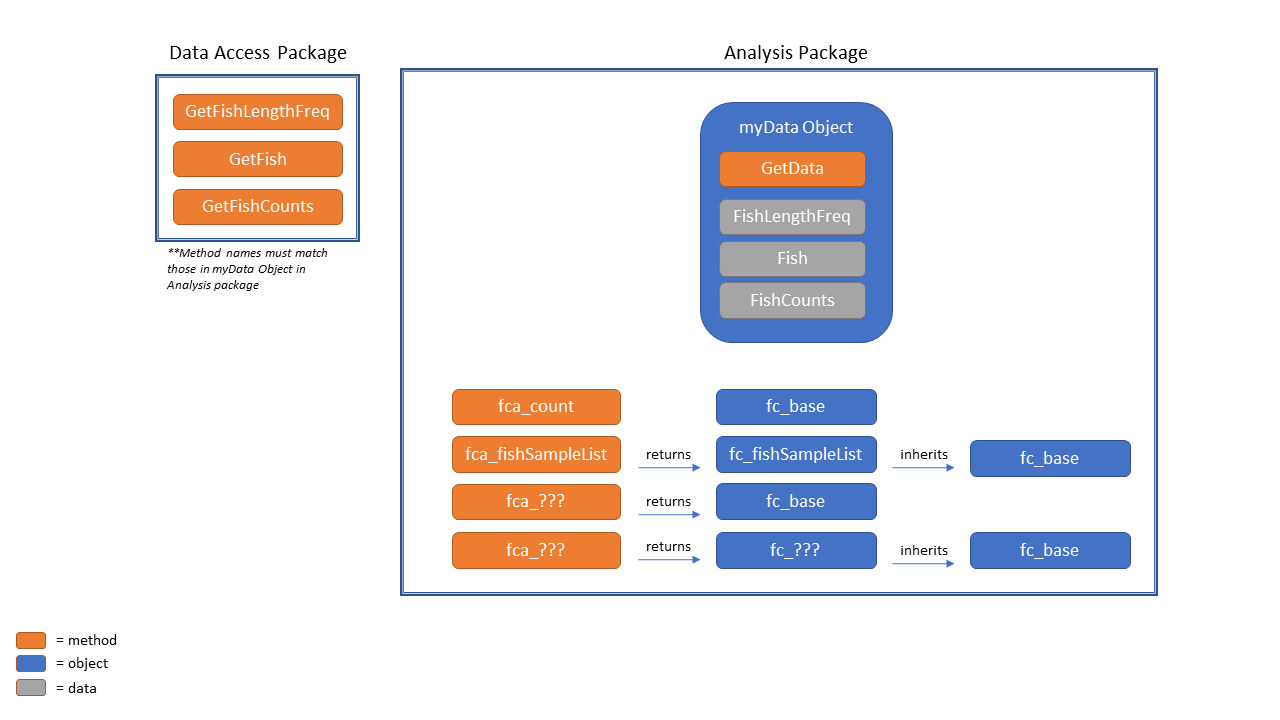
\includegraphics{ArchVis/Slide1.PNG}

\section{WorkFlow}\label{workflow}

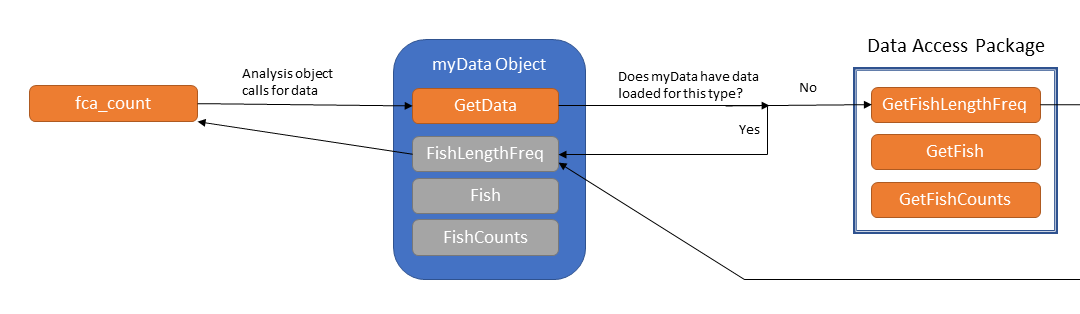
\includegraphics{ArchVis/Slide2.PNG}

\section{Principles}\label{principles}

By Using myData Object:

\begin{itemize}
\item
  Only data that's needed is loaded
\item
  Data is cached
\item
  Data is only retrieved once for entire analysis string
\end{itemize}

By Using Separate Data Access Package:

\begin{itemize}
\item
  Isolates and generalizes data access
\item
  Allows analysis code to use different sources of data
\item
  Allows different scripts to use different authentications for data
  access
\end{itemize}

\chapter{FinCatch Users}\label{fincatch-users}

\section{Auth0 User Authentication}\label{auth0-user-authentication}

FinCatch uses the Auth0 (https://www.auth0.com) for authentication and
authorization. At-will, user-requested new user creation is not
supported. New users can be created by a tenant admin with Auth0. Users
will be sent an email to verify their address and future FinCatch usage
is not possible until the verification is complete. Users should also be
assigned the appropiate authorization roles.

\section{FinCatch User}\label{fincatch-user}

In addition to Auth0 user authentication, FinCatch website, FinCatchAG,
and FinCatchRA users will also need a profile in the FinCatch system.
This profile is meant to decouple FinCatch from the Auth0 system in case
a new authentication service needs to be implemented. Upon the first
login to the FinCatch website, a new Auth0 user with a verified email
will be redirected to a page to create their profile. After creation of
their profile, a FinCatch DataAdmin will need to log in and ``Activate''
their profile.

\section{How to Create A New User}\label{how-to-create-a-new-user}

1) FinCatch administrator logs into Auth0 and creates new user. The
appropiate roles (DataAdmin, DataWorker, DataSupervisor) should be added
to the new user. The new user will need to be supplied their password.

2) New user will receive an email with instructions on how to verify
their email address. The must complete the verification process.

3) New user should log into https://FinCatch.outdoornebraska.gov using
the password supplied by the FinCatch administrator.

4) Upon logging in, the new user will be redirected to a page to
complete their FinCatch profile.

5) A FinCatch administrator must login and activate the new user's
profile.

\part{FinCatchDE}

\chapter{FinCatchDE Deployment}\label{fincatchde-deployment}

\section{\texorpdfstring{\textbf{Before
Deployment}}{Before Deployment}}\label{before-deployment}

Change:

1.~~~~~~ ConnectionString in AppSettings.json

2.~~~~~~ redirectUri at line 45 in previousFishSamples

3. ~~~~~~redirectUri at line 164 in previousWaterSamples

4.~~~~~~ auth0 settings in clsAuthFunctions, fetchController.cs, and
index.tsx

\section{\texorpdfstring{\textbf{Deployment
Steps}}{Deployment Steps}}\label{deployment-steps}

The application needs to be self-contained (See REF-3 and REF-4); you
might want to investigate publishing the application through Visual
Studio's IIS publishing, but this is the way that has worked best for
our development.

1.~~~~~~ Open the Projects in Visual Studio

2.~~~~~~ Ensure the application runs locally through Visual Studio

3.~~~~~~ Right click the solution and select Publish...

4.~~~~~~ Select the Web Server (IIS) Target

5.~~~~~~ Select Web Deploy Package

6.~~~~~~ Put the package location in the same folder as the project

7.~~~~~~ Any name will do for the Site Name, we did Fish-Test, and click
finish

8.~~~~~~ Select Show All Settings

9.~~~~~~ Change Deployment mode to Self-contained

10.~~~ Change the target runtime to the required runtime (for us that
was win-x64)

11.~~~ Select Save

12.~~~ Click the Publish button

13.~~~ Wait for the Publish to be successful

14.~~~ Open the Console/Git Bash/PowerShell

15.~~~ Navigate to
fisheries-field-sampling\textbackslash FisheriesFieldSampling\textbackslash FisheriesFieldSampling\textbackslash client-app\textbackslash~

16.~~~ Run npm run build

17.~~~ Open File Explorer

18.~~~ Navigate to
fisheries-field-sampling\textbackslash FisheriesFieldSampling\textbackslash FisheriesFieldSampling\textbackslash client-app\textbackslash{}

19.~~~ Copy the build folder within the project

20.~~~ Navigate to the newly created zip file from the Publish button

21.~~~ Extract into a folder named publish

22.~~~ Navigate to
publish\textbackslash Content\textbackslash D\_C\textbackslash GitHub\textbackslash fish-test\textbackslash fisheries-field-sampling\textbackslash FisheriesFieldSampling\textbackslash FisheriesFieldSampling\textbackslash obj\textbackslash Release\textbackslash netcoreapp3.1\textbackslash win-x64\textbackslash PubTmp\textbackslash Out\textbackslash client-app
folder

23.~~~ Replace the build folder with the copied build folder

24.~~~ Copy everything within the
publish\textbackslash Content\textbackslash D\_C\textbackslash GitHub\textbackslash fish-test\textbackslash fisheries-field-sampling\textbackslash FisheriesFieldSampling\textbackslash FisheriesFieldSampling\textbackslash obj\textbackslash Release\textbackslash netcoreapp3.1\textbackslash win-x64\textbackslash PubTmp\textbackslash Out\textbackslash{}
folder

25.~~~ Open Remote Desktop

26.~~~ Connect to the fincatchag.fishstaff.info computer

27.~~~ Open the file explorer on the Remote Desktop

28.~~~ Replace the contents of
C:\textbackslash Websites\textbackslash FinCatchDE with the copied
files/folders

29.~~~ Open the IIS Manager

30.~~~ Restart the FinCatchDE website

\part{Analysis R Package}

\chapter{Overview}\label{overview}

\section*{Overview}\label{overview-1}
\addcontentsline{toc}{section}{Overview}

\markright{Overview}

The FinCatchAnalysis (FCA) R package centralizes standard analysis
functions for the FinCatch system and promotes DRY and reusable analysis
code practices. The FCA package is built on top of R6 classes which
provides a standard programming interface for users of the R package.
Analysis functions are available for each individual analysis available
and results from each analysis function returns results encapsulated in
an R6 class object. All public functions in the package are prefixed
with ``fca\_''. Package R6 objects are prefixed with ``fco\_''.

\section{Analysis Functions}\label{analysis-functions}

Each analysis function in the FCA package provides a single call for an
independent analysis and returns a function specific R6 object built on
the base fco\_ object that provides standard methods and data objects.

\section{Analysis Return Objects}\label{analysis-return-objects}

\chapter{Data Object}\label{data-object}

The data object serves a couple of functions. First, it provides a
central method and common approach for data retrieval from the FinCatch
system. It stores the filters used for retrieval and provides a standard
diction for calling the data retrieval functions in the FinCatchAccess
package. Second, it provides a caching mechanism so that during an
analysis chain or report, data will only be downloaded/retrieved from
the database once. Additionally, any commonly used calculations
(i.e.~length-frequency extrapolations) can be defined and cached as
well.

\begin{tcolorbox}[enhanced jigsaw, leftrule=.75mm, coltitle=black, colbacktitle=quarto-callout-warning-color!10!white, colframe=quarto-callout-warning-color-frame, opacitybacktitle=0.6, rightrule=.15mm, colback=white, bottomtitle=1mm, toptitle=1mm, titlerule=0mm, breakable, bottomrule=.15mm, toprule=.15mm, title=\textcolor{quarto-callout-warning-color}{\faExclamationTriangle}\hspace{0.5em}{Warning}, arc=.35mm, opacityback=0, left=2mm]

If the filter objects used in creating the data object change, the data
object should be destroyed and re-created to ensure the cached data and
filters remain synchronized!

\end{tcolorbox}

\section{Creating FinCatch Data
Objects}\label{creating-fincatch-data-objects}

\section{Data Caching And Retrieval}\label{data-caching-and-retrieval}

Data is cached in the ``data\_\ldots{}'' and ``codes\_\ldots{}''
properties of the object. Data and codes are retrieved from the data
object using the ``get\_data\_\ldots{}'' and ``get\_codes\_\ldots{}''
functions. These ``get\_'' functions first check for cached data in the
``data\_'' objects and returns it; otherwise they will retrieve it from
the database, cache it in the ``data\_'' objects, and return it. The
names of ``get\_'' functions match their counterparts in the ``data\_''
objects. The ``data\_'' objects are exposed to users (rather than hiding
them as private objects) so that advanced users can utilize the
FinCatchAnalysis package and the data object by directly saving data to
the cache.

\begin{tcolorbox}[enhanced jigsaw, leftrule=.75mm, coltitle=black, colbacktitle=quarto-callout-important-color!10!white, colframe=quarto-callout-important-color-frame, opacitybacktitle=0.6, rightrule=.15mm, colback=white, bottomtitle=1mm, toptitle=1mm, titlerule=0mm, breakable, bottomrule=.15mm, toprule=.15mm, title=\textcolor{quarto-callout-important-color}{\faExclamation}\hspace{0.5em}{Retrieving Data}, arc=.35mm, opacityback=0, left=2mm]

Data should always be retrieved using ``get\_'' functions, so that
caching works. Trying to retrieve data directly from the ``data\_'' and
``code\_'' cache objects opens up logic errors where lack of data and
yet-to-be retrieved data are confused and confounded.

\end{tcolorbox}

\begin{tcolorbox}[enhanced jigsaw, leftrule=.75mm, coltitle=black, colbacktitle=quarto-callout-caution-color!10!white, colframe=quarto-callout-caution-color-frame, opacitybacktitle=0.6, rightrule=.15mm, colback=white, bottomtitle=1mm, toptitle=1mm, titlerule=0mm, breakable, bottomrule=.15mm, toprule=.15mm, title=\textcolor{quarto-callout-caution-color}{\faFire}\hspace{0.5em}{Caution}, arc=.35mm, opacityback=0, left=2mm]

While data column names may be renamed and table structures combined and
split during caching operations, data should not be modified in any way
that introduce assumptions or potential bias. These type of operations
should use ``get\_calc\_'' and ``calc\_'' names as described below!

\end{tcolorbox}

\section{Calculated Data}\label{calculated-data}

Commonly used calculations are defined in the the data object so that
they do not need to be repeated in the same analysis chain or report.
One example would be length-frequency extrapolations when part of a fish
sample are sub-sampled for length and then extrapolated by fish counts.
These calculations are defined and retrieved in ``get\_calc\_\ldots{}''
functions with their results cached in ``data\_\ldots{}'' objects
similar to the ``data\_'' and ``code\_'' objects.

\section{Warnings and Errors}\label{warnings-and-errors}

Warning and error properties exist in the data object. These accumulate
potential issues encountered when retrieving data/codes from the
database or when performing calculations (such as extrapolated
length-freqencies from a small subsample). These errors are printed to
the console when the FinCatchAnalysis package is used interactively.

\begin{tcolorbox}[enhanced jigsaw, leftrule=.75mm, coltitle=black, colbacktitle=quarto-callout-important-color!10!white, colframe=quarto-callout-important-color-frame, opacitybacktitle=0.6, rightrule=.15mm, colback=white, bottomtitle=1mm, toptitle=1mm, titlerule=0mm, breakable, bottomrule=.15mm, toprule=.15mm, title=\textcolor{quarto-callout-important-color}{\faExclamation}\hspace{0.5em}{Important}, arc=.35mm, opacityback=0, left=2mm]

When the FinCatchAnalysis package is used in a non-interactive
environment like markdown, quarto, or shiny, it is important that these
warnings and errors are explicitly and intentionally shown to the end
user as part of the output!

\end{tcolorbox}

\section{Available Data}\label{available-data}

\section{Available Code}\label{available-code}

\section{Available Calcs}\label{available-calcs}

\chapter{Warnings and Errors}\label{warnings-and-errors-1}

\chapter{Example Script}\label{example-script}

\begin{Shaded}
\begin{Highlighting}[]
\FunctionTok{library}\NormalTok{(FinCatchAccess)}
\FunctionTok{library}\NormalTok{(FinCatchAnalysis)}

\CommentTok{\#use filters gadget to make a filter object}
\NormalTok{myFilters}\OtherTok{\textless{}{-}}\FunctionTok{fcacc\_show\_FilterSelector\_gadget}\NormalTok{()}

\CommentTok{\#feed the filter object with your ID values into a data object}
\NormalTok{myDataObject}\OtherTok{\textless{}{-}}\NormalTok{fc\_data}\SpecialCharTok{$}\FunctionTok{new}\NormalTok{(}\AttributeTok{myFilterObject=}\NormalTok{myFilters, }\AttributeTok{myGroupSurveys=}\ConstantTok{TRUE}\NormalTok{)}

\CommentTok{\#run an analysis by feeding it the data object}
\NormalTok{myAnalysis}\OtherTok{\textless{}{-}}\FunctionTok{fca\_meanLength}\NormalTok{(myDataObject)}

\CommentTok{\#print output tables with printTablesAuto/Html/Latex}
\NormalTok{myAnalysis}\SpecialCharTok{$}\FunctionTok{printTablesAuto}\NormalTok{()}

\CommentTok{\#if you want canned plots}
\NormalTok{myAnalysis}\SpecialCharTok{$}\NormalTok{plots}

\CommentTok{\#view potential data problems}
\NormalTok{myDataObject}\SpecialCharTok{$}\NormalTok{warnings}
\NormalTok{myDataObject}\SpecialCharTok{$}\NormalTok{errors}

\CommentTok{\#view analysis issues}
\NormalTok{myAnalysis}\SpecialCharTok{$}\NormalTok{warnings}
\NormalTok{myAnalysis}\SpecialCharTok{$}\NormalTok{errors}
\end{Highlighting}
\end{Shaded}

\chapter{Base Object}\label{base-object}

\section{Purpose}\label{purpose}

Provides a common interface for results regardless of what analysis is
run.

\subsection{Variables}\label{variables}

\begin{itemize}
\item
  analysisTitle - (string) Description of the analysis stored in the
  object, used for headers and titles in reports and displays
\item
  exportName - (string) Name used when generating file download names,
  no spaces or punctuation should be used
\item
  descriptionText - (string) Markdown text to be displayed in outputs
  prior to the output tables and figures
\item
  tableTitle- (list\textless string\textgreater) Title text to be used
  on object tables, each item in list corresponds to one table output in
  printTables
\item
  groupByVars - (string) Comma-separated string of variable name to use
  as grouping variables within the tables
\item
  surveys - (dataframe) Dataframe containing survey-level data
\item
  samples - (dataframe) Dataframe containing samples
\item
  results - (list\textless dataframes\textgreater) List of dataframes
  containing results of analysis
\item
  plots - (list\textless ggplot objects\textgreater) List of ggPlot
  objects created from analysis
\item
  errors - (list\textless string\textgreater) Error messages created
  during analysis
\item
  warnings- (list\textless string\textgreater) Warning messages created
  during analysis
\item
  groupHeaderBackgroundColor - (string) Color to be used in background
  of group header within table, groups are determined by the groupByVars
  variable, used in HTML outputs only
\item
  groupSummaryBackgroundColor - (string) Color to be used in the summary
  row of each group within table, groups are determined by the
  groupByVars variable, used in HTML outputs only
\item
  gtTheme - (string) Name of gt tables theme from the gtExtras package,
  used in HTML outputs only
\end{itemize}

\subsection{Methods}\label{methods}

\begin{itemize}
\item
  print - method used by R to print the results variable
\item
  exportJson - method used to create and save Json file of results, no
  default implementation
\item
  exportCsv - method used to create and save Csv file of results, no
  default implementation
\item
  createTable - generic table to create both Latex and Html tables for
  object
\item
  createTableLatex - creates table formatted for Latex, default
  implementation simply calls and returns createTable
\item
  createTableHtml - creates table formatted for Html, default
  implementation simply calls and returns createTable
\item
  printTablesLatex - called to output all tables in a LaTex format, this
  does not include any formatting or table specific code which is
  included in the createTable? functions, but instead iterates through
  multiple table outputs
\item
  printTablesHtml - called to output all tables in a Html format, this
  does not include any formatting or table specific code which is
  included in the createTable? functions, but instead iterates through
  multiple table outputs
\item
  printTablesAuto - tests the incoming call for a LaTex environment and
  calls either printTablesLatex or printTablesHtml as appropiate, used
  for markdown reports that can be user-generated in mulitple formats
\item
  iterateSurvey - a generic function that crawls through two loops, one
  for survey groups, one for specific tables (one analysis may output
  mulitiple tables) and is called by the printTable functions
\item
  printPlots - called to output ggplot outputs stored as part of
  analysis
\end{itemize}

\section{Overriding Base Object}\label{overriding-base-object}

The fc\_base object can be extended and customized to produce objects
for specific analysis. See details in ``Creating Analyis Chapter''.

\chapter{Objects}\label{objects}

\section{fc\_counts Object}\label{fc_counts-object}

\section{fc\_fishSampleMedtadata}\label{fc_fishsamplemedtadata}

\chapter{Methods}\label{methods-1}

\section{fca\_counts}\label{fca_counts}

\begin{itemize}
\tightlist
\item
  summarizes number of fish caught in samples by species and gender
\item
  returns fc\_counts object
\end{itemize}

\section{fca\_fishSampleMetadata}\label{fca_fishsamplemetadata}

\begin{itemize}
\tightlist
\item
  returns metadata for fish samples included in analysis
\item
  returns fc\_fishSampleMetadata object
\end{itemize}

\chapter{Helpers}\label{helpers}

There are a number of helper functions available in the FinCatch
Analysis package.

\section{Dplyr Verbs}\label{dplyr-verbs}

\subsection{AddStockCategory}\label{addstockcategory}

This function works as a dplyr verb and adds a column containing a
factor of stock-length categories from Gabelhouse's 5-cell model. The
function takes the name of the column containing the species code, the
column containing the fish length (in mm), and a reference to the data
object for the analysis (needed to retrieve species code and stock
length values). The function defaults to full group names as factor
labels; use abbrieviations=TRUE to use category abbrieviations instead.

Example:

\begin{Shaded}
\begin{Highlighting}[]
\NormalTok{some\_data }\SpecialCharTok{\%\textgreater{}\%}
  \FunctionTok{AddStockCategory}\NormalTok{(sppCode, fishLen, someDataObject, }\AttributeTok{useAbbreviations =} \ConstantTok{TRUE}\NormalTok{) }
\end{Highlighting}
\end{Shaded}

\subsection{AddWrParameters}\label{addwrparameters}

This dplyr verb has yet to be implented

\subsection{AddAgeIntercept}\label{addageintercept}

This dplyr verb has yet to be implemented

\section{Functions}\label{functions}

\subsection{weighted.se.mean}\label{weighted.se.mean}

This function calculates standard error around a weighted mean. The
function assumes a weighted mean calculated by the ``weighted.mean()''
function in the stats package of R and accepts the same arguements.

Example:

\begin{Shaded}
\begin{Highlighting}[]
\NormalTok{some\_data}\OtherTok{=}\FunctionTok{data.frame}\NormalTok{(}\AttributeTok{xValue=}\FunctionTok{c}\NormalTok{(}\DecValTok{3}\NormalTok{,}\DecValTok{4}\NormalTok{,}\DecValTok{6}\NormalTok{,}\DecValTok{3}\NormalTok{,}\DecValTok{2}\NormalTok{,}\DecValTok{3}\NormalTok{),}
                     \AttributeTok{xWeights=}\FunctionTok{c}\NormalTok{(}\FloatTok{0.2}\NormalTok{, }\FloatTok{0.2}\NormalTok{, }\FloatTok{0.3}\NormalTok{, }\FloatTok{0.1}\NormalTok{, }\FloatTok{0.1}\NormalTok{, }\FloatTok{0.1}\NormalTok{))}
\NormalTok{some\_data }\SpecialCharTok{\%\textgreater{}\%}
  \FunctionTok{mutate}\NormalTok{(}\AttributeTok{myWeightedMean=}\FunctionTok{weighted.mean}\NormalTok{(xValue, xWeights, }\AttributeTok{na.rm=}\ConstantTok{TRUE}\NormalTok{),}
         \AttributeTok{myWeightedMeanSE=}\FunctionTok{weighted.se.mean}\NormalTok{(xValue, xWeights, }\AttributeTok{na.rm=}\ConstantTok{TRUE}\NormalTok{))}
\end{Highlighting}
\end{Shaded}

\subsection{fca\_getAnalysisFunctions}\label{fca_getanalysisfunctions}

This function returns a list and description of the analysis functions
available in the FinCatchAnalysis package.

Example:

\begin{Shaded}
\begin{Highlighting}[]
\FunctionTok{fca\_getAnalysisFunctions}\NormalTok{()}
\end{Highlighting}
\end{Shaded}

\section{Labelers}\label{labelers}

\subsection{fc\_labeler\_Survey}\label{fc_labeler_survey}

This function creates a label for each survey to be used in outputs such
as reports and plots. The arguments are a vector of surveyUid values and
a reference to the analysis data object. The label returned is
structured like:

\begin{quote}
Title1 (WB=5110 \textbar{} Method=21 \textbar{} Year=2022 \textbar{}
Season=Spring)
\end{quote}

Example:

\begin{Shaded}
\begin{Highlighting}[]
\NormalTok{some\_data }\SpecialCharTok{\%\textgreater{}\%}
  \FunctionTok{mutate}\NormalTok{(}\AttributeTok{surveyLabel=}\FunctionTok{fc\_labeler\_Survey}\NormalTok{(surveyUid, aDataObject))}
\end{Highlighting}
\end{Shaded}

\subsection{fc\_labeler\_fishSample}\label{fc_labeler_fishsample}

This function creates a label for each fish sample to be used in outputs
such as reports and plots. The arguments are a vector of surveyUid
values and a dataframe of fish samples in the analysis taken from the
data object. The label returned is structured like:

\begin{quote}
WB=2832 \textbar{} Method=45 \textbar{} 2022-03-11 \textbar{}
Station=627
\end{quote}

Example:

\begin{Shaded}
\begin{Highlighting}[]
\NormalTok{some\_data }\SpecialCharTok{\%\textgreater{}\%}
  \FunctionTok{mutate}\NormalTok{(}\AttributeTok{sampleLabel=}\FunctionTok{fc\_labeler\_fishSample}\NormalTok{(surveyUid, aDataObject}\SpecialCharTok{$}\NormalTok{get\_data\_samplesFish))}
\end{Highlighting}
\end{Shaded}

\subsection{fc\_labeler\_wqSample}\label{fc_labeler_wqsample}

This function creates a label for each fish sample to be used in outputs
such as reports and plots. The arguments are a vector of surveyUid
values and a dataframe of fish samples in the analysis taken from the
data object. The label returned is structured like:

\begin{quote}
WB=2832 \textbar{} 2022-03-11 \textbar{} Station=627
\end{quote}

Example:

\begin{Shaded}
\begin{Highlighting}[]
\NormalTok{some\_data }\SpecialCharTok{\%\textgreater{}\%}
  \FunctionTok{mutate}\NormalTok{(}\AttributeTok{sampleLabel=}\FunctionTok{fc\_labeler\_wqSample}\NormalTok{(surveyUid, aDataObject}\SpecialCharTok{$}\NormalTok{get\_data\_samplesWq))}
\end{Highlighting}
\end{Shaded}

\subsection{fc\_matchCodes}\label{fc_matchcodes}

www

\subsection{fc\_createCodeLabel}\label{fc_createcodelabel}

www

\subsection{fc\_createCodeLabelReversed}\label{fc_createcodelabelreversed}

www

\chapter{Create Analysis}\label{create-analysis}

\subsection{General}\label{general}

Analysis function calls are prefixed with ``fca\_'' and object names are
prefixed with ``fc\_''

Make sure to test each analysis function for:

\begin{itemize}
\item
  Data selected by surveys only
\item
  Data selected by samples only
\item
  Data selected by both surveys and samples
\item
  Filters that return NO data
\item
  Species in processing list and not in data
\item
  Species not in processing list and in data
\item
  Works for both grouped by survey and ungrouped analysis, if not
  grouped by survey in fc\_data\$groupSurveys, surveyUid is set to
  ``-1'' during data download by the data object
\end{itemize}

\subsection{Flow and Critical Issues}\label{flow-and-critical-issues}

\begin{itemize}
\item
  Import Data

  \begin{itemize}
  \item
    Make sure to use remove\_nonCPUE\_data as appropiate in get\_data\_
    functions

    \begin{tcolorbox}[enhanced jigsaw, leftrule=.75mm, coltitle=black, colbacktitle=quarto-callout-important-color!10!white, colframe=quarto-callout-important-color-frame, opacitybacktitle=0.6, rightrule=.15mm, colback=white, bottomtitle=1mm, toptitle=1mm, titlerule=0mm, breakable, bottomrule=.15mm, toprule=.15mm, title=\textcolor{quarto-callout-important-color}{\faExclamation}\hspace{0.5em}{Important}, arc=.35mm, opacityback=0, left=2mm]

    use remove\_nonCPUE\_data=FALSE to get all data if appropriate,
    specify remove\_nonCPUE\_data=TRUE for readability (is default if
    not specified)

    \end{tcolorbox}
  \item
    Check For Empty/Missing Stations using ??? function
  \end{itemize}
\item
  Conduct Analysis

  \begin{itemize}
  \tightlist
  \item
    Expand to account for missing 0's using AddZerosForMissingSpecies()
    function
  \end{itemize}
\item
  Finish Analysis

  \begin{itemize}
  \item
    Label survey UIDs, sample UIDs, species, and methods
  \item
    \begin{tcolorbox}[enhanced jigsaw, leftrule=.75mm, coltitle=black, colbacktitle=quarto-callout-note-color!10!white, colframe=quarto-callout-note-color-frame, opacitybacktitle=0.6, rightrule=.15mm, colback=white, bottomtitle=1mm, toptitle=1mm, titlerule=0mm, breakable, bottomrule=.15mm, toprule=.15mm, title=\textcolor{quarto-callout-note-color}{\faInfo}\hspace{0.5em}{Note}, arc=.35mm, opacityback=0, left=2mm]

    Useful Functions:

    fc\_labeler\_Survey

    fc\_labeler\_fishSample

    fc\_labeler\_wqSample

    fc\_matchCodes

    fc\_createCodeLabel

    fc\_createCodeLabelReversed

    \end{tcolorbox}
  \end{itemize}
\end{itemize}

\subsection{Steps}\label{steps}

\begin{enumerate}
\def\labelenumi{\arabic{enumi}.}
\item
  Create new r file names fc\_analysisName.R (Easiest To Copy Existing
  Analysis and Modify)
\item
  No library statements should be included in R file. Instead, they need
  to be included in the package DESCRIPTION file.
\item
  Create/Modify the roxygen comments for procedure
\item
  Name/Rename function. Analysis functions are prefixed with ``fca\_''
  and the same base name as the ``fc\_'' file.
\item
  All function calls require a FinCatch Data Object (fc\_data) to be
  passed to an arguement named ``myData''
\item
  Check that fish (or Wq) samples exist in the current dataset.
\item
  Set grouping variables.
\end{enumerate}

\begin{itemize}
\tightlist
\item
  To group analysis calculations during analysis, use the dplyr verbs
\end{itemize}

\begin{Shaded}
\begin{Highlighting}[]
        \FunctionTok{group\_by}\NormalTok{(}\FunctionTok{across}\NormalTok{(}\FunctionTok{all\_of}\NormalTok{(myGroups))}
\end{Highlighting}
\end{Shaded}

\begin{itemize}
\tightlist
\item
  add addition fields as necessary ``group\_by(across(all\_of(myGroups),
  anotherFieldHere)''
\end{itemize}

\begin{enumerate}
\def\labelenumi{\arabic{enumi}.}
\setcounter{enumi}{7}
\tightlist
\item
  Write analysis code
\end{enumerate}

\begin{itemize}
\item
  Always include Standard Error and Sample size (if appropriate), this
  allow users to calculate difference confidence intervals post hoc
\item
  When including confidence intervals, include 95\% and 80\%
\item
  Make sure to account for missing data in any input
\end{itemize}

\begin{enumerate}
\def\labelenumi{\arabic{enumi}.}
\setcounter{enumi}{8}
\tightlist
\item
  Label values like survey, sample, species, waterbody, etc.
\end{enumerate}

\begin{itemize}
\item
  Labelers exist for samples and surveys (make sure surveyUid's are set
  to -1 if not grouping by survey
\item
  Helper functions are available for coded values
\end{itemize}

\begin{enumerate}
\def\labelenumi{\arabic{enumi}.}
\setcounter{enumi}{9}
\item
  If analysis is calculated (as opposed to raw data summations), screen
  out species NOT in the processing list. This is necessisary because
  species NOT in the list do not carry the assumption that all specimans
  for that species were processed.
\item
  Attach all results to an analysis object (either base or custom).
  Example:
\end{enumerate}

\begin{Shaded}
\begin{Highlighting}[]
    \CommentTok{\#create return object at beginning of function }
\NormalTok{    (this allows errors and warnings to be added throughout survey)}
\NormalTok{    op }\OtherTok{\textless{}{-}}\NormalTok{ fc\_meanWeight}\SpecialCharTok{$}\FunctionTok{new}\NormalTok{()}
\NormalTok{    op}\SpecialCharTok{$}\NormalTok{analysisTitle }\OtherTok{=} \StringTok{"Mean Weight (Weighted)"}
\NormalTok{    op}\SpecialCharTok{$}\NormalTok{exportName }\OtherTok{=} \StringTok{"MeanWeight"}
\NormalTok{    op}\SpecialCharTok{$}\NormalTok{descriptionText }\OtherTok{=} \StringTok{"These results display weighted mean }
\StringTok{                          weight.  Calculations are weighted as }
\StringTok{                          only a non{-}proportional (i.e. first 10 fish }
\StringTok{                          per 10mm length group) number of fish }
\StringTok{                          are subsampled."}
\NormalTok{    op}\SpecialCharTok{$}\NormalTok{tableTitle }\OtherTok{\textless{}{-}} \FunctionTok{list}\NormalTok{(}\StringTok{"Weighted Mean Weight"}\NormalTok{)}
\NormalTok{    op}\SpecialCharTok{$}\NormalTok{groupByVars }\OtherTok{\textless{}{-}} \StringTok{"speciesCode"}
\NormalTok{    op}\SpecialCharTok{$}\NormalTok{groupSurveys }\OtherTok{\textless{}{-}}\NormalTok{ myData}\SpecialCharTok{$}\NormalTok{groupSurveys}
    
    \CommentTok{\#during function, add warnings and errors to return object}
\NormalTok{    op}\SpecialCharTok{$}\NormalTok{errors }\OtherTok{\textless{}{-}}\NormalTok{ rlist}\SpecialCharTok{::}\FunctionTok{list.append}\NormalTok{(op}\SpecialCharTok{$}\NormalTok{errors, }\StringTok{"Error1 Message"}\NormalTok{, }\StringTok{"Error2 Message"}\NormalTok{)}
\NormalTok{    op}\SpecialCharTok{$}\NormalTok{warnings }\OtherTok{\textless{}{-}}\NormalTok{ rlist}\SpecialCharTok{::}\FunctionTok{list.append}\NormalTok{(op}\SpecialCharTok{$}\NormalTok{warnings, }\StringTok{"Warning1"}\NormalTok{)}
    
    \CommentTok{\#at end of function, add results to return object}
\NormalTok{    op}\SpecialCharTok{$}\NormalTok{results }\OtherTok{\textless{}{-}} \FunctionTok{list}\NormalTok{(}\FunctionTok{data.frame}\NormalTok{(d))}
\NormalTok{    op}\SpecialCharTok{$}\NormalTok{plots }\OtherTok{\textless{}{-}}\NormalTok{ myPlots}
    
\end{Highlighting}
\end{Shaded}

\begin{enumerate}
\def\labelenumi{\arabic{enumi}.}
\setcounter{enumi}{11}
\tightlist
\item
  Add the function to the list of analysis functions available in the
  package (found in inst folder). This list is used to populate the
  FinCatchRA UI and to feed the fc\_getAvailableAnalysis function.
\end{enumerate}

\subsection{Create Custom Analysis R6
Object}\label{create-custom-analysis-r6-object}

All analysis results are returned using R6 objects. This allows for
consistent use and implementation of different analysis functions by
parent applications and code. A base R6 object, ``fc\_base'', provides
all the basic functions and structure for FinCatch analysis objects.
Custom objects can be created in the analysis files to allow customized
output tables and plots and MUST inherit from the fc\_base object.

Column names will often need to be altered to provided user friendly
text in the outputs. In addition, sometimes valuable columns are dropped
for display purposes. Both of these should be done in the analysis
output object createTable functions, NOT in the analysis function itself
or in the ``results'' property of the output object. This is to provide
for consistency between analyses and is important for the download
function of FinCatchRA.

Every effort is made to ensure tables produced by analysis objects work
in both HTML (which allows more formatting options and used by
FinCatchRA) and in LaTex (for PDF report generation). Basic table
creation should happen by providing a ``CreateTable'' function. Any
additional work needed for specific HTML or LaTex output should be
included in overridden ``CreateTableHtml'' or ``CreateTableLatex''
functions\ldots.which otherwise just call and return the ``CreateTable''
function by default.

\begin{Shaded}
\begin{Highlighting}[]
\NormalTok{fc\_counts }\OtherTok{\textless{}{-}} \FunctionTok{R6Class}\NormalTok{(}\StringTok{"fc\_counts"}\NormalTok{,}
                    \AttributeTok{inherit =}\NormalTok{ fc\_base,}
                    \AttributeTok{public =} \FunctionTok{list}\NormalTok{(}
                      \AttributeTok{createTable =} \ControlFlowTok{function}\NormalTok{(mySurveyUid, myTableNumber) \{}
                          \CommentTok{\#if data was selected by samples only…all surveyUids will be blank}
\NormalTok{                      op }\OtherTok{\textless{}{-}} \ConstantTok{NA}

\NormalTok{                      thisSurveyLabel }\OtherTok{\textless{}{-}}\NormalTok{ (self}\SpecialCharTok{$}\NormalTok{results[[myTableNumber]] }\SpecialCharTok{\%\textgreater{}\%}                                 \FunctionTok{filter}\NormalTok{(surveyUid }\SpecialCharTok{==}\NormalTok{ mySurveyUid) }\SpecialCharTok{\%\textgreater{}\%}
                        \FunctionTok{pull}\NormalTok{(surveyLabel))[[}\DecValTok{1}\NormalTok{]]}
                        
\NormalTok{                      op }\OtherTok{\textless{}{-}}\NormalTok{ self}\SpecialCharTok{$}\NormalTok{results[[myTableNumber]] }\SpecialCharTok{\%\textgreater{}\%}
                        \FunctionTok{filter}\NormalTok{(surveyUid }\SpecialCharTok{==}\NormalTok{ mySurveyUid) }\SpecialCharTok{\%\textgreater{}\%}
                        \FunctionTok{group\_by}\NormalTok{(countSpeciesLabel, sampleLabel) }\SpecialCharTok{\%\textgreater{}\%}
                        \FunctionTok{summarise}\NormalTok{(}\AttributeTok{FishCount =} \FunctionTok{sum}\NormalTok{(FishCount, }\AttributeTok{na.rm =} \ConstantTok{TRUE}\NormalTok{)) }\SpecialCharTok{\%\textgreater{}\%}
                        \FunctionTok{mutate}\NormalTok{(}\AttributeTok{countGenderLabel =} \StringTok{"Total"}\NormalTok{) }\SpecialCharTok{\%\textgreater{}\%}
                        \FunctionTok{bind\_rows}\NormalTok{(self}\SpecialCharTok{$}\NormalTok{results[[myTableNumber]]  }\SpecialCharTok{\%\textgreater{}\%}
                        \FunctionTok{filter}\NormalTok{(surveyUid }\SpecialCharTok{==}\NormalTok{ mySurveyUid)) }\SpecialCharTok{\%\textgreater{}\%}
                        \FunctionTok{arrange}\NormalTok{(countSpeciesLabel, sampleLabel, countGenderLabel) }\SpecialCharTok{\%\textgreater{}\%}
                        \FunctionTok{select}\NormalTok{(}\SpecialCharTok{{-}}\NormalTok{countSpeciesCode,}\SpecialCharTok{{-}}\NormalTok{countGenderCode,}\SpecialCharTok{{-}}\NormalTok{sampleUid,}\SpecialCharTok{{-}}\NormalTok{surveyLabel,}\SpecialCharTok{{-}}\NormalTok{surveyUid) }\SpecialCharTok{\%\textgreater{}\%} 
                        \FunctionTok{spread}\NormalTok{(countGenderLabel, FishCount, }\AttributeTok{fill =} \DecValTok{0}\NormalTok{) }\SpecialCharTok{\%\textgreater{}\%}
                        \FunctionTok{relocate}\NormalTok{(}\StringTok{"Total"}\NormalTok{, }\AttributeTok{.after =} \FunctionTok{last\_col}\NormalTok{()) }\SpecialCharTok{\%\textgreater{}\%}
                        \FunctionTok{gt}\NormalTok{(}\AttributeTok{rowname\_col =} \FunctionTok{colnames}\NormalTok{(self}\SpecialCharTok{$}\NormalTok{results[[}\DecValTok{1}\NormalTok{]])[}\DecValTok{8}\NormalTok{]) }\SpecialCharTok{\%\textgreater{}\%}
                          \FunctionTok{tab\_options}\NormalTok{(}
                            \AttributeTok{row\_group.background.color =}\NormalTok{ self}\SpecialCharTok{$}\NormalTok{groupHeaderBackgroundColor,}
                            \AttributeTok{summary\_row.background.color =}\NormalTok{ self}\SpecialCharTok{$}\NormalTok{groupSummaryBackgroundColor}
\NormalTok{                            ) }\SpecialCharTok{\%\textgreater{}\%} 
                          \FunctionTok{tab\_header}\NormalTok{(}\AttributeTok{title =} \FunctionTok{md}\NormalTok{(self}\SpecialCharTok{$}\NormalTok{tableTitle),}
                                    \AttributeTok{subtitle =}\NormalTok{ thisSurveyLabel) }\SpecialCharTok{\%\textgreater{}\%}
                          \FunctionTok{summary\_rows}\NormalTok{(}\AttributeTok{groups =} \ConstantTok{TRUE}\NormalTok{,}
                                      \AttributeTok{columns =} \FunctionTok{everything}\NormalTok{(),}
                                      \AttributeTok{fns =} \FunctionTok{list}\NormalTok{(}\StringTok{"Total"} \OtherTok{=} \StringTok{"sum"}\NormalTok{),}
                                      \AttributeTok{formatter =}\NormalTok{ fmt\_integer,}
                                      \AttributeTok{use\_seps =} \ConstantTok{TRUE}\NormalTok{,}
                                      \AttributeTok{missing\_text =} \StringTok{""}\NormalTok{) }\SpecialCharTok{\%\textgreater{}\%}
\NormalTok{                          self}\SpecialCharTok{$}\FunctionTok{gtTheme}\NormalTok{()}
                          
                        \FunctionTok{return}\NormalTok{(op)}
\NormalTok{                      \}}
\NormalTok{                    ))}
\end{Highlighting}
\end{Shaded}

\part{Data Access R Package}

\section*{Packages}\label{packages-1}
\addcontentsline{toc}{section}{Packages}

\markright{Packages}

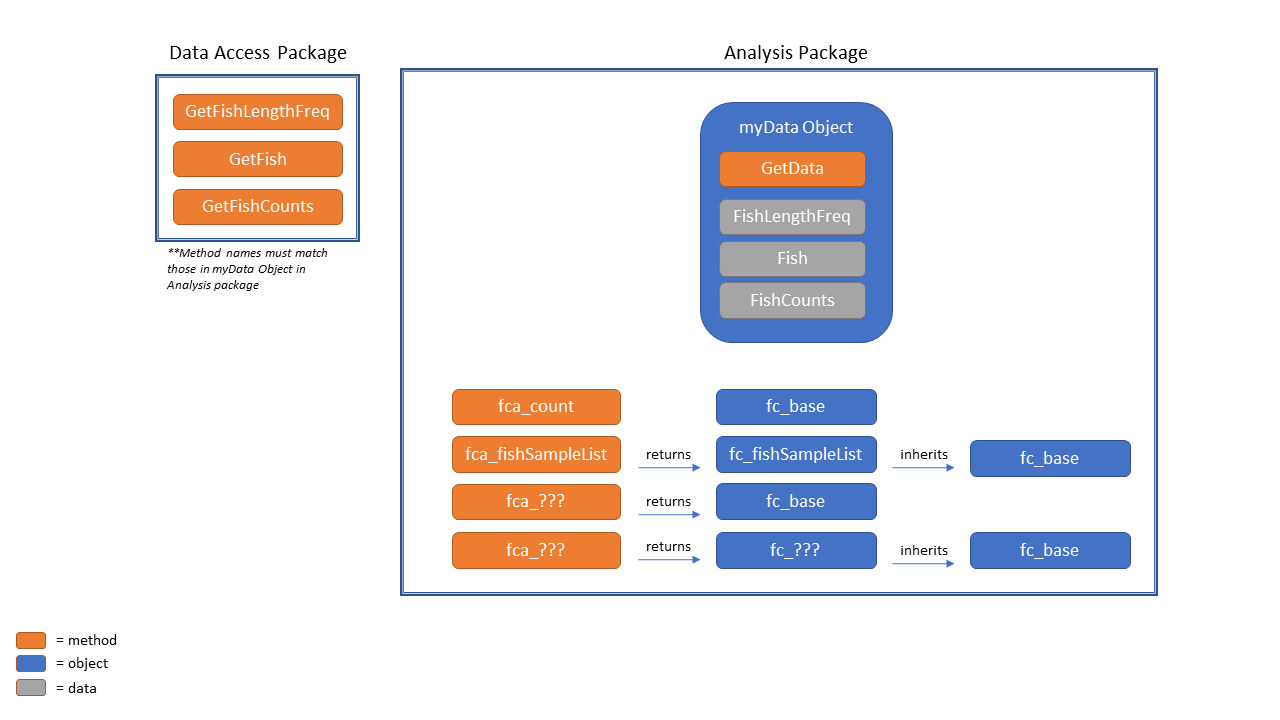
\includegraphics{ArchVis/Slide1.PNG}

\section*{WorkFlow}\label{workflow-1}
\addcontentsline{toc}{section}{WorkFlow}

\markright{WorkFlow}

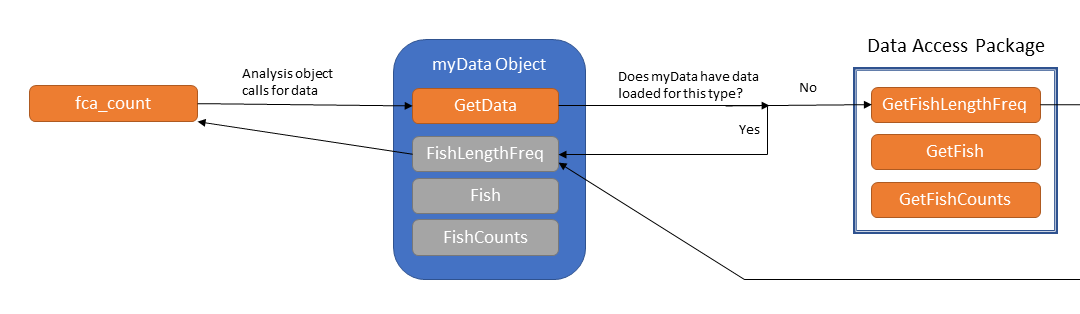
\includegraphics{ArchVis/Slide2.PNG}

\section*{Principles}\label{principles-1}
\addcontentsline{toc}{section}{Principles}

\markright{Principles}

By Using myData Object:

\begin{itemize}
\item
  Only data that's needed is loaded
\item
  Data is cached
\item
  Data is only retrieved once for entire analysis string
\end{itemize}

By Using Separate Data Access Package:

\begin{itemize}
\item
  Isolates and generalizes data access
\item
  Allows analysis code to use different sources of data
\item
  Allows different scripts to use different authentications for data
  access
\end{itemize}

\part{References}

\phantomsection\label{refs}
\begin{CSLReferences}{0}{1}
\end{CSLReferences}



\end{document}
